
\documentclass[%
 reprint,
%superscriptaddress,
%groupedaddress,
%unsortedaddress,
%runinaddress,
%frontmatterverbose, 
%preprint,
%preprintnumbers,
%nofootinbib,
%nobibnotes,
%bibnotes,
 amsmath,amssymb,
 aps,
%pra,
%prb,
%rmp,
%prstab,
%prstper,
%float,
]{revtex4-2}
\usepackage{url}
\usepackage{float}
\usepackage{graphicx}% Include figure files
\usepackage{dcolumn}% Align table columns on decimal point
\usepackage{bm}% bold math
%\usepackage{hyperref}% add hypertext capabilities
%\usepackage[mathlines]{lineno}% Enable numbering of text and display math
%\linenumbers\relax % Commence numbering lines

%\usepackage[showframe,%Uncomment any one of the following lines to test 
%%scale=0.7, marginratio={1:1, 2:3}, ignoreall,% default settings
%%text={7in,10in},centering,
%%margin=1.5in,
%%total={6.5in,8.75in}, top=1.2in, left=0.9in, includefoot,
%%height=10in,a5paper,hmargin={3cm,0.8in},
%]{geometry}

\begin{document}

\preprint{APS/123-QED}

\title{Measurement of the Speed of Light in Air with Laser Pulses}% Force line breaks with \\

\author{Dean Reiter}
\affiliation{%
 Cornell University\\
}%

\date{\today}% It is always \today, today,
             %  but any date may be explicitly specified

\begin{abstract}
The speed of light in air at standard temperature and pressure is experimentally measured to be $c = 3.0160 \times 10^8 \pm 3.00 \times 10^6$ m/s with a $1\sigma$ confidence level, agreeing with the known value within 0.633 standard deviations of uncertainty. The difference in time-of-flight between laser pulses travelling different path lengths in a Michelson interferometer is measured by analyzing the statistically-averaged signals produced by the laser pulses incident on a photon detector.

\end{abstract}

%\keywords{Suggested keywords}%Use showkeys class option if keyword
                              %display desired
\maketitle

%\tableofcontents

\section{Introduction}

The speed of electromagnetic radiation, $c$, is a fundamental constant in relativistic physics which scientists have strived to measure since the 17th century. The Danish astronomer Roemer first measured $c$ in 1675 by analyzing variations in the orbit of Jupiter's moons, while in the 19th century, experiments by Fizeau and Foucault refined the measurement using the timing of rotating wheels and mirrors \cite{french}. By the late 20th century, technological leaps in precision culminated in the 1983 redefinition of $c$ in vacuum as exactly 299,792,458 m/s, a fundamental constant from which the unit of the meter is now derived \cite{NIST_meter}.

A Michelson interferometer is an optical instrument that splits a beam of light into two perpendicular paths, reflects them off mirrors, and then recombines them to form an interference pattern. Originally used by Albert Michelson in 1881 to search for the luminiferous ether, the interferometer played a crucial role in the development of special relativity by proving the invariance of the speed of light. In such an apparatus, a path length difference between the two arms introduces a flight-time delay and corresponding phase shift between the beams, resulting in a measurable interference pattern \cite{french}\cite{Michelson1881relative}\cite{Michelson1887On}. Rather than measuring the interference created by a steady-state light source as in the traditional setup, the experiment presented aims to measure the speed of light using a pulsed source and measuring the flight-time delay in a Michelson interferometer directly. 



\section{Experimental Setup}

The optical setup pictured in Fig. 1 is similar to a Michelson interferometer, but it is not used to measure an interference pattern. The red laser used is similar to a commercial, low-power laser pointer, and its effective power is reduced to 0.56 mW by a polarizing filter, which is not shown in Fig. 1. The laser beam travels 20 cm before passing through a beam splitter. One of the split beams travels a short path, passing through another polarizing filter (not shown in Fig. 1) and reflecting off a mirror, which is 19.50 $\pm$ 0.25 cm away, before returning to the beam splitter. The other split beam travels a long path, reflecting off a parabolic mirror, which is 10.490 $\pm$ 0.101 m away from the beam splitter, and four times between that mirror and another, which is a distance of 10.235 $\pm$ 0.101 m from the first, before finally returning to the beam splitter. The redirected beams travel a final 37 cm before entering a photomultiplier tube. The overall path length difference, $\Delta x$, between the long and short paths is 102.47 $\pm$ 1.02 m. 

\begin{figure}[H]
\centering
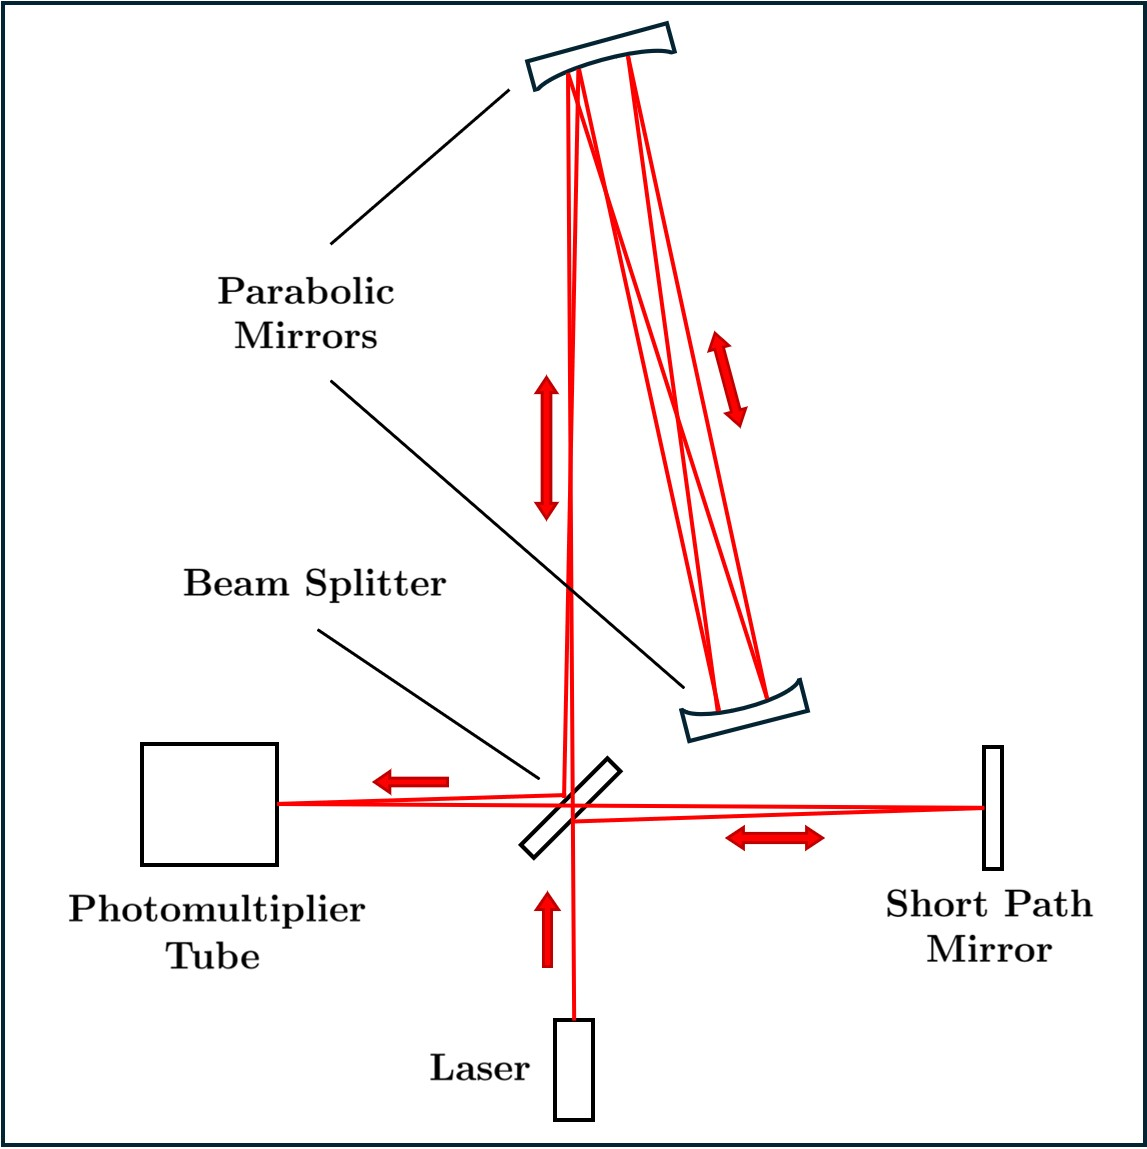
\includegraphics[width=0.75\columnwidth]{Diagram.jpg}% Here is how to import EPS art
\caption{\label{fig:epsart} Optical setup in which a laser beam is split into two paths. The beam traveling the long path reflects five times between parabolic mirrors positioned 10 meters away before returning to the beam splitter, resulting in a total path length that is 102.45 $\pm$ 1.02 m longer than that of the beam which travels the short path. The split paths are recombined and directed to a photomultiplier which measures light intensity.}
\end{figure}

The electronic equipment consists of a high-voltage DC power supply, a photomultiplier tube, a voltage amplifier, a Systron Donner 101 Pulse Generator, and a Tektronix TBS 2000B Series Digital Oscilloscope. The photomultiplier tube, which is given a 900 V supply, produces an electrical current when it detects photons from the laser beam. The photomultiplier output is amplified by 50 dB and measured by the oscilloscope. The pulse generator supplies the laser with square-wave voltage pulses with a width of 3.0 $\pm$ 0.1 $\mu$s at a frequency of 1.0 kHz. This is the shortest pulse width that can activate the laser diode, which is not designed to be pulsed for extremely short durations. A reference signal from the pulse generator, which is proportional to the signal it supplies the laser, triggers the oscilloscope. Since the photomultiplier output is highly sensitive, the oscilloscope records the average of 512 trigger cycles of the photomultiplier signal to reduce noise.

The optical setup was adjusted to perform measurements of the long-path and short-path beams individually. An opaque plate was positioned to obstruct either the short path or the long path as desired to measure the beam which travels each path in isolation. Due to the unknown time-dependence of the photomultiplier and amplifier's electrical response to light intensity, the polarizing filter between the beam splitter and short path mirror (not shown in Fig. 1) was calibrated so that the difference between the average signal amplitude of the short and long-path beams is less than 50 mV.

\section{Data and Analysis}

The intensities as a function of time of the laser beam pulses which travel the two paths in the optical setup in Fig. 1 were measured by a photomultiplier. The intensities of the long-path and short-path beams were each measured in isolation by individually obstructing the beam paths. The amplified laser pulse signals produced by the photomultiplier were averaged over 512 pulse cycles of 1 kHz and recorded by an oscilloscope. Each waveform recording contains 20 thousand averaged measurements of the voltage of the amplified photomultiplier signal over a duration of 20 $\mu$s. The averages of 10 oscilloscope recordings of each laser pulse signal are shown in Fig. 2. 

\begin{figure}[H]
\centering
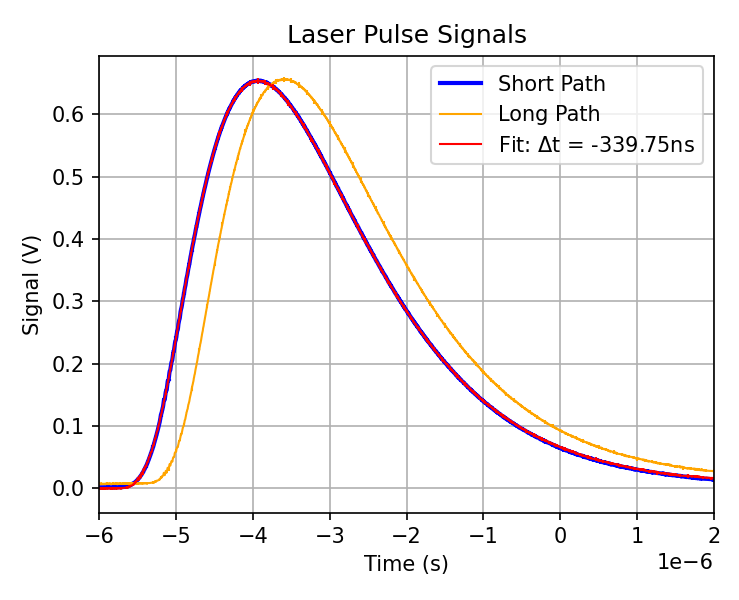
\includegraphics[width=0.9\columnwidth]{Signals2.png}% 
\caption{\label{fig:epsart} An 8 $\mu$s selection of the averaged electrical signals produced by laser pulses which traveled the long path (yellow) and by those which traveled the short path (blue) in the apparatus in Fig. 1. The long-path signal is advanced by 339.75 ns and fitted to the short-path signal (red). Each signal shown is the average of 5,120 pulses. The error bars shown are too small to distinguish. }
\end{figure}

 A non-linear least squares minimization is used to fit the averaged long-path signal to the averaged short-path signal \cite{scipy}. The fitted data is shown in red in Fig. 2. The timescale of the oscilloscope data, which is triggered by the pulse generator at 1 kHz, is used as an objective timescale by which to compare the long-path and short-path signals. The ends of the short-path signal are cut, and we define the short-path signal to be the set of 1,899 voltage measurements: $\left\{t_i, y_i  \pm \sigma_{y_i}\right\}$, $t_i \in [-9.5,9.5]\text{ }\mu\text{s}$. The function $f(t, \vec{\theta})$ estimates and transforms the long-path signal as a continuous function of time, $t$, by linearly interpolating the discrete long-path signal data, which we define as the set: $\left\{t_i, x_i  \pm \sigma_{x_i}\right\}$, $t_i \in [-10,10]\text{ }\mu\text{s}$. The fitting parameters, $\vec{\theta} = (a,b,\delta)$, linearly transform the long-path signal to model the expected physical time-shift, $\Delta t = \delta$, an amplitude differential, $a$, and a difference in average signal background, $b$.

\begin{equation}
    f(t, \vec{\theta}) = \begin{cases}
    a x_i + b\text{,}  & t - \delta = t_i, \\
    a \left[\frac{x_{i+1} - x_{i}}{t_{i+1} - t_{i}} (t-t_i-\delta) + x_i\right] + b\text{,} & t_i < t - \delta < t_{i+1}.
    \end{cases}
\end{equation}

\noindent We define a similar continuous function to estimate the standard deviation of the long-path signal for interpolated measurements:

\begin{equation}
    \sigma_f(t, \vec{\theta}) = \begin{cases}
    a \sigma_{x_i}\text{,}  & t - \delta = t_i, \\
    a \left[\frac{\sigma_{x_{i+1}} - \sigma_{x_{i}}}{t_{i+1} - t_{i}} (t-t_i-\delta) + \sigma_{x_i}\right]\text{,} & t_i < t - \delta < t_{i+1}.
    \end{cases}
\end{equation}

\noindent The fitting program determines the parameters $\vec{\theta}$ which minimize the chi-squared statistic,

\begin{equation}
    \chi^2 = \sum_{i=0}^{1899} \frac{\left(y_i - f(t_i, \vec{\theta})\right)^2}{\sigma_{y_i}^2 + \sigma_f^2(t_i,\vec{\theta})}.
\end{equation}

\noindent The standard variances, $\vec{s}_\theta=(\sigma_a^2, \sigma_b^2, \sigma_{\delta}^2)$, of the parameters determined by the chi-squared minimization are estimated to be the diagonal elements of the covariance matrix from the minimization method, weighted by the reduced chi-squared. The covariance matrix can be computed from the Jacobian matrix, $J$, output by the minimization program, so the estimated variances of the fitting parameters are given by

\begin{equation}
    \vec{s}_\theta = \text{diag}\left(\frac{\chi^2}{1896} \left[J^T J \right]^{-1}  \right) \cite{Turley2018}.
\end{equation}

The long-path signal is fit to the short-path signal with the parameters $a = 1.00837 \pm 9 \times 10^{-5}$, $b = -8.12925 \times 10^{-3} \pm  1.244 \times 10^{-5} $, and $\delta = 3.39753 \times 10^{-7 } \pm  9.6 \times 10^{-11}$. The residuals of the fit are shown in Fig. 3. The time delay between the arrival of the short-path and long-path laser pulses is therefore measured to be $\Delta t = 339.753 \pm 0.096$ ns, and the speed of light in air (Eq. 1) is measured to be $c = 3.0160 \times 10^8 \pm 3.00 \times 10^6$ m/s.

\begin{figure}[H]
    \centering
    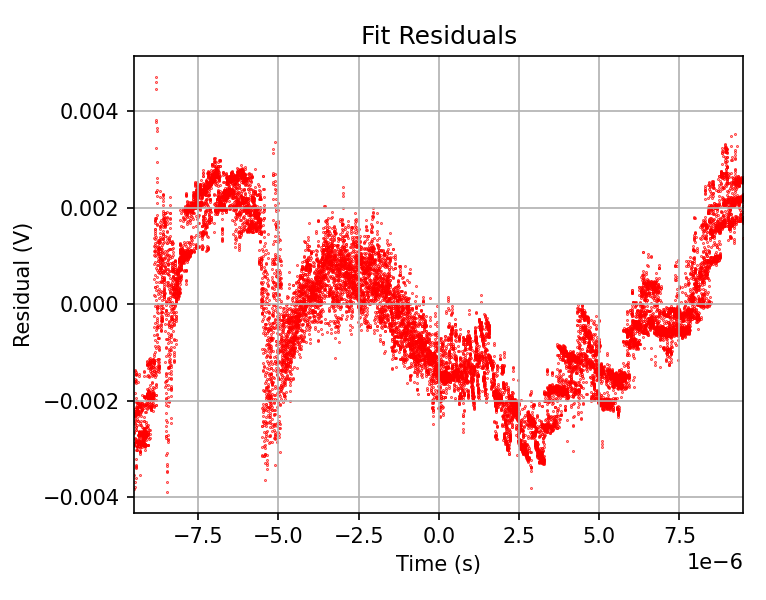
\includegraphics[width=0.9\columnwidth]{Residuals.png}% 
    \caption{\label{fig:epsart} The residuals between the short-path beam signal, $y_i$, and the fitted long-path beam signal, $f(t, \vec{\theta})$. The even pattern around the peak of the pulse signal at $t = -3.5$ $\mu$s suggests that the three-parameter fit is unable to completely model the physics in the experiment.}
    \end{figure}

The greatest source of error in this measurement is the $1\%$ uncertainty in the length of the long path of the optical setup, which results from the fact that the 10 meter distances between the parabolic mirrors, and between the far parabolic mirror and the beam splitter, could not be measured easily with the tools available. The distances were measured as a combination of parallel distances along the laboratory table and distances along the laboratory floor, and only a single meter stick and measuring tape were used. The uncertainty in the distance between the parabolic mirrors is then amplified by an order of magnitude in the total length of the long path. Discontinuities in the distance measurement therefore introduced uncertainties which could be remedied in the future by utilizing a single measurement tool and more precise procedure. 

The electrical sensitivity of the photomultiplier and amplifier is a clear source of statistical uncertainty. It was necessary to average the photomultiplier signal over 512 pulse cycles in the oscilloscope, but the shape of the averaged waveform still visibly fluctuates during the course of a measurmement. Taking the average of 10 oscilloscope recordings improved the precision of the waveform, but the precision will improve with the square root of the number of recordings. Recording at least an order of magnitude more waveforms, possibly utilizing an automated system, could therefore greatly improve the measurement precision.

Given the clear non-Gaussian pattern in the residual plot, there must be unknown systematic errors in the experiment which the three-parameter fit model does not capture. Specifically, the residual plot exhibits an even pattern around the peak of the pulse signal, between -5.0 $\mu$s and 0.0 $\mu$s, as shown in Fig. 3. The photomultiplier and amplifier could be the source of this additional systematic error if they exhibit unwanted and unkown electrical response characteristics which are time-dependent and could alter the shape of the pulse waveforms, such as rising-edge delays, falling-edge delays, or signal saturation. Another potential but likely insignficant source of systematic error is dispersion of the long-path beam in air, which would cause different frequencies of light in the beam to travel at different phase velocities and result in a wider pulse signal. Lasers are highly coherent by design, however, so frequncy dispersion of the long-path beam may not be significant in this experiment.  

\section{Conclusion}


The speed of light in air is measured to be $3.0160 \times 10^8$ m/s within a $1\sigma$ confidence interval from $2.9860 \times 10^8$ m/s to $3.0460 \times 10^8$ m/s. The exact measurement is 0.634 percent greater than the known value of the speed of light in air, $2.9970 \times 10^8$ m/s, but it agrees within 0.633 standard deviations. The measurement of the speed of light with this apparatus can be improved by reducing the uncertainty in the distance measurements, reducing the statistical uncertainty in the time delay measurment, and by determining and then correcting unknown systematic uncertainties.    


\bibliography{main}% Produces the bibliography via BibTeX.

\end{document}
%
% ****** End of file apssamp.tex ******
